\documentclass[a4paper,11pt]{amsart}
\usepackage{pgf,tikz,pgfplots}
\pgfplotsset{compat=1.15}
\usepackage{mathrsfs}
\usetikzlibrary{arrows}
\pagestyle{empty}

\usepackage{amssymb}
\usepackage{graphicx}
\usepackage{tkz-graph}

\parskip 1ex
\parindent 0 pt

\newcounter{temp}
\newcounter{prob_counter}
\newcounter{sprob_counter}

\newenvironment{problem}
{\begin{list}{{\bf \arabic{prob_counter}}}{
      \usecounter{prob_counter}
      \addtolength{\labelsep}{.6ex}
      \addtolength{\itemsep}{4.3ex}
      \setlength{\leftmargin}{1.4em}}
      \setcounter{prob_counter}{\value{temp}}
}
{\setcounter{temp}{\value{prob_counter}}
  \end{list}
}

\newenvironment{subprob}
{
  \begin{list}{{\bf \alph{sprob_counter}}}{
      \usecounter{sprob_counter}
      \addtolength{\labelsep}{.6ex}
      \addtolength{\itemsep}{.5ex}
      \setlength{\leftmargin}{1.7em}}
}
{\end{list}}

\newenvironment{solution}{\textbf{Solution.}}{\qed}

\newcommand{\rubrik}[1]{\bigskip \begin{center}{\bf #1}\end{center} \medskip}

\newcommand{\NN}{\mathbb{N}}
\newcommand{\ZZ}{\mathbb{Z}}
\newcommand{\QQ}{\mathbb{Q}}
\newcommand{\RR}{\mathbb{R}}


\tikzset{
  VertexStyle/.append style = {draw, circle, minimum size=0.125cm, inner sep=0.25cm}
}


\begin{document}
\definecolor{rvwvcq}{rgb}{0.08235294117647059,0.396078431372549,0.7529411764705882}

\pagestyle{empty}
\thispagestyle{empty}

{\small{\sc\noindent
        Arnaldur Bjarnason ({\tt arnaldur15@ru.is}) and Árni Dagur ({\tt arnidg@protonmail.ch})
}}

\rubrik{PROBLEM SET 2 (T-445-GRTH)}

You need to collect $\bf 65$ points to get a full score {\bf but} you cannot get more than {\bf X} points (in total) from a problem section with annotation {\bf max X}.

{\bf Please make sure to:}\\
1. Write your name/email(s) above.\\
2. Write your answers in \texttt{{\textbackslash}begin\{solution\} ... {\textbackslash}end\{solution\}} blocks given after each problem. Turn in a single \LaTeX-generated pdf.\\
3. Write clear and concise proofs: points may be deducted for vagueness.



\section{Trees ({\bf max 45})}

\begin{problem}
 \item (5 points) Let $T$ be a tree with at least 3 vertices.
 Is it true that the complement of $T$ is connected unless $T$ is a star?
\end{problem}
\begin{solution}
  Let $\overline{G}$ be the complement of $G$. For $\overline{G}$ to have two disconnected components, $G$ must have a subgraph $S$ where $V(S) = V(G)$ that is a complete bipartite graph $S = K_{m,n}$. If $m = 1 \lor n = 1$ then $S$ is a star and if $m > 1$, $S$ has a cycle and is thus not a tree.
\end{solution}

\begin{problem}
 \item (15 points) State necessary and sufficient conditions on an ordered $n$-tuple of positive integers
 $(d_1, \dots, d_n)$ with $d_1 \le d_2 \le \dots \le d_n$ in order that there be a tree $T$ on vertices $u_1, \dots, u_n$
 with $\text{deg}_T(u_i) = d_i$ for each $i \in \{1, \dots, n \}$.
\end{problem}
\begin{solution}
  \begin{itemize}
  \item $\forall i \in \{1, \dots, n \} : d_i \geq 1$.
  \item $\displaystyle\sum_{v \in V(T)}{\text{deg}_T(v)} = \sum_{i\in \{1,\dots,n\}}d_i = 2|V(T)|-2$
  \end{itemize}
  To maintain these conditions, there must always be at least two $i : d_i = 1$ and there can be an arbitrary amount of $i : d_i = 2$.\\
  $\forall i : d_i > 2$ there are $d_i-2$ unique $j : d_j = 1$
\end{solution}

\begin{problem}
\item \begin{subprob}
  \item (5 points) Let $(v_1, v_2, \ldots, v_n)$ be a sequence on $n \geq 1$ distinct objects.
  For $j = 2, \ldots, n$, let $i(j)$ be an index in $\{1, \ldots, j-1\}$.
  Show that the simple graph $G$ with $V(G) = \{v_1, v_2, \ldots, v_n\}$ and $E(G) = \{v_2v_{i(2)}, v_3v_{i(3)}, \ldots, v_nv_{i(n)}\}$ is a tree.
\item (10 points) Let $T$ be a tree.
Prove that there exists a permutation $(v_1, v_2, \ldots, v_n)$ of $V(T)$ with the following property: for $j = 2, \ldots, n$, vertex $v_j$ is adjacent to exactly one vertex in the set $\{v_1, \ldots, v_{j-1}\}$.
\end{subprob}
\end{problem}
\begin{solution}

\end{solution}

\begin{problem}
  \item (10 points) Let $P$, $Q$ and $R$ be three paths on a tree $T$.
  Suppose that $V(P) \cap V(Q) \neq \emptyset$, $V(Q) \cap V(R) \neq \emptyset$, and $V(P) \cap V(R) \neq \emptyset$.
  Prove that $V(P) \cap V(Q) \cap V(R) \neq \emptyset$.
\end{problem}
\begin{solution}
  Let $P = \{p_1, ..., c_1, ..., c_3, ..., p_a\}$,
  $Q = \{q_1, ..., c_1, ..., c_2, ..., q_b\}$, and
  $R = \{r_1, ..., c_2, ..., c_3, ..., r_c\}$. Where $c_1$, is a vertex where
  $P$ and $Q$ intersect, $c_2$ where $Q$ and $R$ intersect, and
  $c_3$ where $P$ and $R$ intersect.

  Let's observe the graph that we get by intersecting P and Q through $c_1$:

  \begin{center} % {{{
    \begin{tikzpicture}[line cap=round,line join=round,>=triangle 45,x=1cm,y=1cm]
      \begin{axis}[
        x=1cm,y=1cm,
        axis lines=none,
        ymajorgrids=false,
        xmajorgrids=false,
        xmin=-8.8,
        xmax=-1.5,
        ymin=1.5,
        ymax=8.8,
        xtick={},
        ytick={},]
        \draw [line width=2pt] (-6,4)-- (-6,5);
        \draw [line width=2pt] (-6,5)-- (-6,6);
        \draw [line width=2pt] (-7,4)-- (-6,4);
        \draw [line width=2pt] (-8,4)-- (-7,4);
        \draw [line width=2pt] (-6,4)-- (-5,4);
        \draw [line width=2pt] (-5,4)-- (-4,4);
        \draw [line width=2pt] (-4,4)-- (-3,4);
        \draw [line width=2pt] (-6,7)-- (-6,6);
        \draw [line width=2pt] (-6,4)-- (-6,3);
        \draw [line width=2pt] (-6,3)-- (-6,2);
        \draw [line width=2pt] (-6,7)-- (-6,8);
        \draw [line width=2pt] (-3,4)-- (-2,4);
        \begin{scriptsize}
          \draw [fill=rvwvcq] (-6,4) circle (2.5pt);
          \draw[color=rvwvcq] (-5.84,4.43) node {$c_1$};
          \draw [fill=rvwvcq] (-6,5) circle (2.5pt);
          \draw[color=rvwvcq] (-5.84,5.43) node {$...$};
          \draw [fill=rvwvcq] (-6,6) circle (2.5pt);
          \draw[color=rvwvcq] (-5.84,6.43) node {$c_2$};
          \draw [fill=rvwvcq] (-7,4) circle (2.5pt);
          \draw[color=rvwvcq] (-6.84,4.43) node {$...$};
          \draw [fill=rvwvcq] (-8,4) circle (2.5pt);
          \draw[color=rvwvcq] (-7.84,4.43) node {$p_1$};
          \draw [fill=rvwvcq] (-5,4) circle (2.5pt);
          \draw[color=rvwvcq] (-4.84,4.43) node {$...$};
          \draw [fill=rvwvcq] (-4,4) circle (2.5pt);
          \draw[color=rvwvcq] (-3.84,4.43) node {$c_3$};
          \draw [fill=rvwvcq] (-3,4) circle (2.5pt);
          \draw[color=rvwvcq] (-2.84,4.43) node {$...$};
          \draw [fill=rvwvcq] (-6,7) circle (2.5pt);
          \draw[color=rvwvcq] (-5.84,7.43) node {$...$};
          \draw [fill=rvwvcq] (-6,3) circle (2.5pt);
          \draw[color=rvwvcq] (-5.84,3.43) node {$...$};
          \draw [fill=rvwvcq] (-6,2) circle (2.5pt);
          \draw[color=rvwvcq] (-5.84,2.43) node {$q_1$};
          \draw [fill=rvwvcq] (-6,8) circle (2.5pt);
          \draw[color=rvwvcq] (-5.84,8.43) node {$q_b$};
          \draw [fill=rvwvcq] (-2,4) circle (2.5pt);
          \draw[color=rvwvcq] (-1.84,4.43) node {$p_a$};
        \end{scriptsize}
      \end{axis}
    \end{tikzpicture}
  \end{center} % }}}
  Remember that the verteces $c_2$ and $c_3$ both belong to the path $R$. To
  avoid creating a cycle (no cycles are allowed in trees!) R must go through
  $c_1$. Ergo, $c_1$ belongs to all three paths.
\end{solution}

\begin{problem}
  \item (10 points) Let $\Delta \ge 3$, and let $d_{\Delta}(n)$ be the maximum number of nodes
 of degree $\Delta$ that a tree on $n$ vertices may have. Use induction to show that:
 \[
  d_{\Delta}(n) \le \left \lfloor \frac{n-2}{\Delta - 1} \right \rfloor.
 \]
\end{problem}
\begin{solution}
\end{solution}

\begin{problem}
\item \begin{subprob}
  \item (10 points) Show that if a tree $T$ has a longest path of even length, then the mid-vertex of one such longest path is the mid-vertex of every longest path in $T$. {\tiny Hint: First show that two such paths can't be vert.-disjoint.}
\item (5 points) Prove that the common vertex is a center of $T$.
\end{subprob}
\end{problem}
\begin{solution}
\end{solution}

\newpage
\begin{problem}
 \item (5 points) A full ternary tree is an ordered rooted tree where each vertex, except the leaves, has
 exactly $3$ children. Hence, all of the internal vertices have degree four, except the root which has degree
 $3$. Prove the \textit{Full Ternary Tree Theorem} which states that a full ternary tree has $n = 3k+1$ vertices,
 $k$ of them internal and $2k+1$ of them leaves.
\end{problem}
\begin{solution}
  Let's prove this by induction on $n$. Let $X(n)$ be the number of external
  verteces in a full ternary tree with $n$ internal nodes.

  \textbf{Base case:}
  \[
    X(0) = 1 = 2n + 1
  \]

  \textbf{Induction step:}
  Suppose our hypothesis is true for $\forall i < n$. Our root has three
  branches. Let $a$ and $b$ be the number of internal verteces belonging to the
  leftmost and middle branches, respectively. The last branch then has $n - a -
  b - 1$ internal verteces. From this follows:
 \begin{align*}
    X(n) =
    \\X(a) + x(b) + X(n - a - b - 1) =
    \\2a + 1 + 2b + 1 + 2(n - a - b - 1) + 1 =
    \\2n + 1
  \end{align*}
\end{solution}



\newpage
\section{Spanning Trees ({\bf max 10})}

\begin{problem}
 \item (5 points) Describe a procedure for finding a spanning tree in a graph. Prove that it indeed finds a spanning tree in every connected graph. Apply it to the graph from the following exercise.
\end{problem}
\begin{solution}
  Start by picking any vertex and adding it to $T$. \\
  Then pick any edge $\{u,v\} \in E(G), u \notin V(T), v \in V(T)$.
  If $V(G) = V(T), T$ is the spanning tree of $G$,
  otherwise if $\{u,v\} \notin E(G)$, $G$ has no spanning tree,
  otherwise add $\{u,v\}$ to $E(T)$ and $u$ to $V(T)$. \\
  \\
  Let $N$ be a connected graph whose spanning tree the procedure doesn't find.
  There must be $\forall u : u \in V(N), u \notin V(T), d(u) \geq 1$ there is an edge $\{u,v\} \in E(N), \{u,v\} \notin E(T), v \notin V(T)$. There must then be a path from $u$ to all $v \in V(N)$ and thus $\forall v \in V(N), v \notin V(T)$ which is a contradiction as $V(T) \subseteq V(N)$ and is not empty if $V(N) \neq N_0$. \\
  Here is the graph with the steps of the procedure enumerated.
  \[
  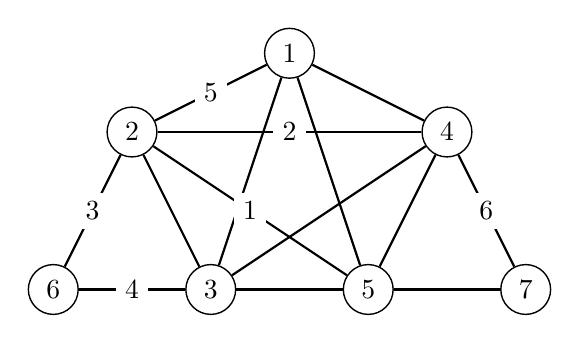
\begin{tikzpicture}
    \GraphInit[vstyle=normal]
    \SetGraphUnit{3}
    \Vertex[x=3,y=3]{1}
    \Vertex[x=1,y=2]{2}
    \Vertex[x=5,y=2]{4}
    \Vertex[x=2,y=0]{3}
    \Vertex[x=4,y=0]{5}
    \Vertex[x=0,y=0]{6}
    \Vertex[x=6,y=0]{7}

    \Edge[color=blue,label=5](1)(2)
    \Edge(1)(3)
    \Edge(1)(4)
    \Edge(1)(5)
    \Edge(2)(3)
    \Edge[color=blue,label=2](2)(4)
    \Edge[color=blue,label=1](2)(5)
    \Edge(3)(4)
    \Edge(3)(5)
    \Edge(4)(5)
    \Edge[color=blue,label=3](2)(6)
    \Edge[color=blue,label=4](3)(6)
    \Edge[color=blue,label=6](4)(7)
    \Edge(5)(7)
  \end{tikzpicture}
\]
And here is the resulting tree.
\[
  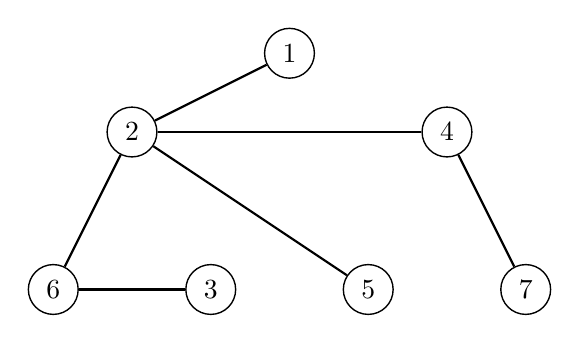
\begin{tikzpicture}
    \GraphInit[vstyle=normal]
    \SetGraphUnit{2}
    \Vertex[x=3,y=3]{1}
    \Vertex[x=1,y=2]{2}
    \Vertex[x=5,y=2]{4}
    \Vertex[x=2,y=0]{3}
    \Vertex[x=4,y=0]{5}
    \Vertex[x=0,y=0]{6}
    \Vertex[x=6,y=0]{7}

    \Edge(1)(2)
    \Edge(2)(4)
    \Edge(2)(5)
    \Edge(2)(6)
    \Edge(3)(6)
    \Edge(4)(7)
  \end{tikzpicture}\\
\]
\end{solution}

\newpage
\begin{problem}
 \item (10 points) How many different spanning trees does the following graph contain?
\begin{center}
 \includegraphics[height=4cm]{st-count.pdf}
\end{center}
\end{problem}
\begin{solution}
  We begin by taking the degree matrix $D(G)$ and adjacency matrix $A(G)$ and by the Matrix-Tree theorem we have $\det(C(D(G) - A(G))) = nsp$ where $C$ is a function that removes the first row and column of a matrix, $\det$ is the determinant and $nsp$ is the number of spanning trees
  \[
    D(G) =
    \begin{bmatrix}
      4&0&0&0&0&0&0 \\
      0&5&0&0&0&0&0 \\
      0&0&5&0&0&0&0 \\
      0&0&0&5&0&0&0 \\
      0&0&0&0&5&0&0 \\
      0&0&0&0&0&2&0 \\
      0&0&0&0&0&0&2 \\
    \end{bmatrix}
    A(G) =
    \begin{bmatrix}
      0&1&1&1&1&0&0 \\
      1&0&1&1&1&1&0 \\
      1&1&0&1&1&1&0 \\
      1&1&1&0&1&0&1 \\
      1&1&1&1&0&0&1 \\
      0&1&1&0&0&0&0 \\
      0&0&0&1&1&0&0 \\
    \end{bmatrix}
  \]\\
  \[
    C(D(G)-A(G))=
    \begin{bmatrix}
      5&-1&-1&-1&-1&0 \\
      -1&5&-1&-1&-1&0 \\
      -1&-1&5&-1&0&-1 \\
      -1&-1&-1&5&0&-1 \\
      -1&-1&0&0&2&0 \\
      0&0&-1&-1&0&2 \\
    \end{bmatrix}
  \] \\
  \[
    det(C(D(G) - A(G))) = \underline{720}
  \]
  There are 720 spanning trees in $G$.
\end{solution}

\newpage
\section{Eulerian Graphs ({\bf max 25})}

\begin{problem}
\item
 Consider the $3 \times 3$ chessboard, and let $Q$ denote the $9$ squares of the board. Let
 $H_{3,3} = (Q, E)$ denote the simple graph on vertex set $Q$ so that $(q_1, q_2) \in E$ if and
 only if a rook at square $q_1$ can reach $q_2$ in a single move (a rook can move
 horizontally and vertically  arbitrary distance).
\begin{subprob}
 \item (5 points) Run \textit{Fleury's algorithm} for computing an Eulerian circuit on $H_{3,3}$. The algorithm on a simple graph $G=(V,E)$ is as follows:
 \begin{quote}
 Pick a vertex $v_1$ arbitrarily. Having picked $v_1, \dots, v_k$,  set
 $G_k = G \, - \, \{e_{1,2}, e_{2,3}, \dots, e_{{k-2},{k-1}}, e_{{k-1},k} \}$, where $e_{i,j}$ denotes
 an edge connecting $v_i$ to $v_j$.
 If there is a non-bridge (in $G_k$) edge connecting $v_k$ to a vertex $u$ then let
 $v_{k+1} = u$. Otherwise, let $v_{k+1}$ be any neighbor of $v_k$ in $G_k$. If the degree of $v_k$ in
 $G_k$ is $0$ then terminate. Repeat.
 \end{quote}

\item  (5 points) Consider the general $n \times m$ chessboard, for $n,m \ge 1$, and similarly the graph $H_{n,m}$ so that two vertices (squares) are adjacent if and only if a rook can get from one to the other in one move. For which values $n,m$ does the graph $H_{m,n}$ contain a Euler circuit?
 \item (10 points) Prove that Fleury's algorithm always finds an Eulerian circuit if there is one.
 \end{subprob}
\end{problem}
\begin{solution}
  \begin{subprob}
  \item On the left in the following figure is an image of the graph
    $H_{3,3}$ and on the right, each edge has been labeled with an
    index $i$ where $i$ is the $i$th edge in a eulerian cycle on $G$.
  \[
    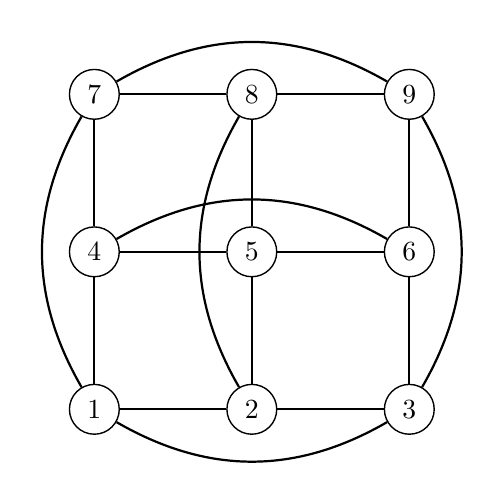
\begin{tikzpicture}[x=2cm,y=2cm]
      \GraphInit[vstyle=normal]
      \SetGraphUnit{4}
      \Vertex[x=0,y=0]{1} \Vertex[x=1,y=0]{2} \Vertex[x=2,y=0]{3} \Vertex[x=0,y=1]{4} \Vertex[x=1,y=1]{5} \Vertex[x=2,y=1]{6} \Vertex[x=0,y=2]{7} \Vertex[x=1,y=2]{8} \Vertex[x=2,y=2]{9}

      \Edge(1)(2) \Edge[style={bend right}](1)(3) \Edge(1)(4) \Edge[style={bend left}](1)(7) \Edge(2)(3) \Edge(2)(5) \Edge[style={bend left}](2)(8) \Edge(3)(6) \Edge[style={bend right}](3)(9) \Edge(4)(5) \Edge[style={bend left}](4)(6) \Edge(4)(7) \Edge(5)(6) \Edge(5)(8) \Edge(6)(9) \Edge(7)(8) \Edge[style={bend left}](7)(9) \Edge(8)(9)
    \end{tikzpicture}
    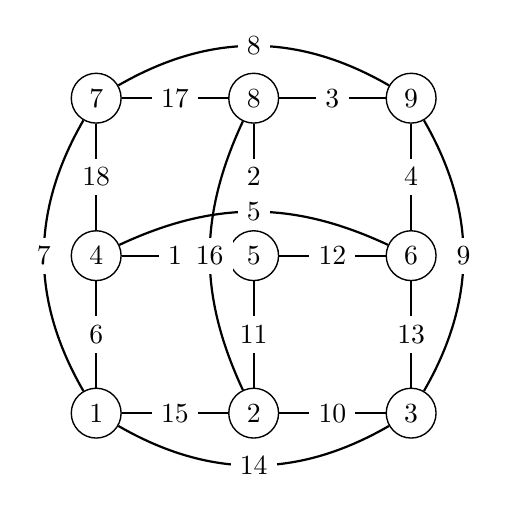
\begin{tikzpicture}[x=2cm,y=2cm]
      \GraphInit[vstyle=normal]
      \SetGraphUnit{2}
      \Vertex[x=0,y=0]{1} \Vertex[x=1,y=0]{2} \Vertex[x=2,y=0]{3} \Vertex[x=0,y=1]{4} \Vertex[x=1,y=1]{5} \Vertex[x=2,y=1]{6} \Vertex[x=0,y=2]{7} \Vertex[x=1,y=2]{8} \Vertex[x=2,y=2]{9}

      \Edge[label=15](1)(2) \Edge[label=14,style={bend right}](1)(3) \Edge[label=6](1)(4) \Edge[label=7,style={bend left}](1)(7) \Edge[label=10](2)(3) \Edge[label=11](2)(5) \Edge[label=13](3)(6) \Edge[label=9,style={bend right}](3)(9) \Edge[label=1](4)(5) \Edge[label=18](4)(7) \Edge[label=12](5)(6) \Edge[label=2](5)(8) \Edge[label=4](6)(9) \Edge[label=17](7)(8) \Edge[label=8,style={bend left}](7)(9) \Edge[label=3](8)(9) \Edge[label=16,style={bend left=25}](2)(8) \Edge[label=5,style={bend left=25}](4)(6)
    \end{tikzpicture}\\
  \]
  The description for Fleury's algorithm is absolute nonsense, I don't know what it's saying even though I understand the algorithm.

\item $\forall v \forall u : d_H(v) = d_H(u)$ where $H = H_{n,m}$ for any $m,n \in \NN$. $d_{H_{n,m}}(v) = n+m-2$ which can easily be proven by induction. Since by theorem 5.7 in the book: a connected graph $G$ is Eulerian iff each vertex in $G$ has even degree. Therfore $H_{n,m}$ has a Eulerian cycle if $m+n$ is even.
\end{subprob}

\end{solution}


\begin{problem}
\item (10 points) For an integer $k$, let $G$ be a connected graph that contains $2k$ vertices of odd degree. Show that there exist $k$ edge-disjoint subgraphs $G_1, \dots, G_k$ such that
 \begin{itemize}
  \item $E(G) = E(G_1) \cup E(G_2) \cup \dots \cup E(G_k)$,
  \item each $G_i$ has an Eulerian trail.
 \end{itemize}

\tiny{Hint: Add $k$ edges to $G$ so that it becomes Eulerian.}
\end{problem}
\begin{solution}
\end{solution}


\begin{problem}
\item (5 points) Prove that a balanced weakly connected digraph is strongly connected.
\end{problem}
\begin{solution}
  Let $\overrightarrow{G}$ be a weakly connected digraph. Theorem 5.25 in the book states that $\overrightarrow{G}$ is balanced if and only if it
  is Eulearian — that is, it has a Eulerian cycle. It of course doesn't matter what vertex
  we start from in a Eulerian cycle, we can always get to every other vertex.
  From that follows that $\overrightarrow{G}$ is strongly connected.
\end{solution}



\section{Hamiltonian and Bipartite Graphs ({\bf max 22})}



\begin{problem}
 \item Let $m$ and $n$ be positive integers. Consider the \textit{grid graph} $G_{m,n} = (V, E)$ with vertex set $V = \{1, \dots, m\} \times \{1, \dots, n\}$, where vertices $u = (x, y) \in V$ and $v = (x', y') \in V$ are adjacent if and only if $|x - x'| + |y - y'| = 1$.
 \begin{subprob}
  \item (5 points) Show that grid graphs are bipartite, for all $m, n \geq 1$.
  \item (10 points) Find necessary and sufficient conditions that $m$ and $n$ must satisfy in order for the graph $G_{m,n}$ to be Hamiltonian.
 \end{subprob}
\end{problem}
\begin{solution}
  \begin{subprob}
  \item The adjacency formula of $G_{m,n}$ describes the fact that the sum of the coordinates of each neighbour of vertex $v$ differs by exactly one.
    Let $v=(x,y) \in G$ be even if $x+y$ is even and odd if the opposite is true.
    This means that $\{u,v\} \in E \Longrightarrow \text{odd}(u) \oplus \text{odd}(v)$ meaning that either $v$ or $u$ is odd but not both.
    The vertices can be partitioned into partitions of even vertices and another of odd vertices that satisfy the properties of bipartite graphs.
  \item Let $S \subset G_{m,n}$ be the set of odd vertices. It should be obvious that $|G_{m,n}| = mn$ and it follows that $G_{m,n}-S=N_{\lceil \frac{mn}{2} \rceil}$ where $N_n$ is the null graph of size $n$. This is true since removing all vertices from a partition in a bipartite graph, leaves a null graph with the size of the number of vertices in the remaining partition. $|S| = \lfloor \frac{mn}{2} \rfloor$.\\
    By theorem 5.16 one can see that when $mn$ is odd, the division by two causes $|S| < \left| N_{\lceil \frac{mn}{2} \rceil}\right|$ which means that the graph is not Hamiltonian. If $mn$ is even, the opposite applies and G is Hamiltonian.
  \end{subprob}

\end{solution}

\newpage
\begin{problem}
\item (7 points) Prove that the following graph is not Hamiltonian.
  \begin{center}
    \includegraphics[height=5cm]{hamiltonian.pdf}
  \end{center}
\end{problem}
\begin{solution}
  Theorem 5.16 states that if $G$ is a simple hamiltonian graph, then for each $S \subseteq V(G)$, the number of components of $G - S$ is at most $|S|$.
  By removing 6 vertices, we are left with 7 components as can be seen in the two figures, and thus G is not Hamiltonian.
  \[
    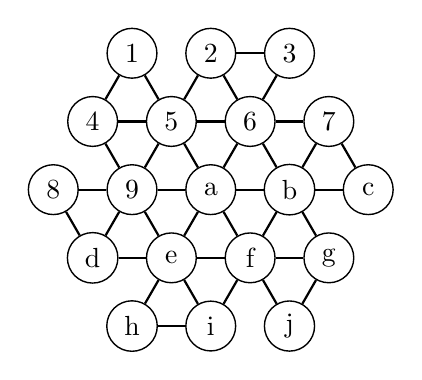
\begin{tikzpicture}[x=0.5cm,y=0.866025cm]
      \GraphInit[vstyle=normal]
      \Vertex[x=2,y=0]{1}
      \Vertex[x=4,y=0]{2}
      \Vertex[x=6,y=0]{3}
      \Vertex[x=1,y=-1]{4}
      \Vertex[x=3,y=-1]{5}
      \Vertex[x=5,y=-1]{6}
      \Vertex[x=7,y=-1]{7}
      \Vertex[x=0,y=-2]{8}
      \Vertex[x=2,y=-2]{9}
      \Vertex[x=4,y=-2]{a}
      \Vertex[x=6,y=-2]{b}
      \Vertex[x=8,y=-2]{c}
      \Vertex[x=1,y=-3]{d}
      \Vertex[x=3,y=-3]{e}
      \Vertex[x=5,y=-3]{f}
      \Vertex[x=7,y=-3]{g}
      \Vertex[x=2,y=-4]{h}
      \Vertex[x=4,y=-4]{i}
      \Vertex[x=6,y=-4]{j}

      \Edge(1)(4)
      \Edge(1)(5)
      \Edge(2)(3)
      \Edge(2)(5)
      \Edge(2)(6)
      \Edge(3)(6)
      \Edge(4)(5)
      \Edge(4)(9)
      \Edge(5)(6)
      \Edge(5)(9)
      \Edge(5)(a)
      \Edge(6)(7)
      \Edge(6)(a)
      \Edge(6)(b)
      \Edge(7)(b)
      \Edge(7)(c)
      \Edge(8)(9)
      \Edge(8)(d)
      \Edge(9)(a)
      \Edge(9)(d)
      \Edge(9)(e)
      \Edge(a)(b)
      \Edge(a)(e)
      \Edge(a)(f)
      \Edge(b)(c)
      \Edge(b)(f)
      \Edge(b)(g)
      \Edge(d)(e)
      \Edge(e)(f)
      \Edge(e)(h)
      \Edge(e)(i)
      \Edge(f)(g)
      \Edge(f)(j)
      \Edge(f)(i)
      \Edge(g)(j)
      \Edge(h)(i)
    \end{tikzpicture} \ \
    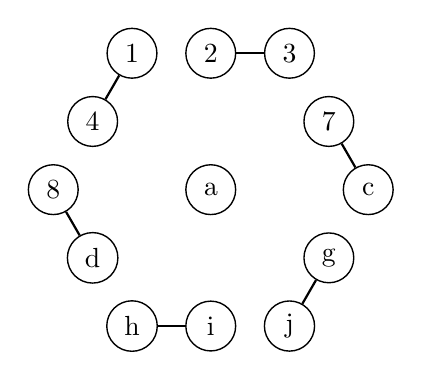
\begin{tikzpicture}[x=0.5cm,y=0.866025cm]
      \GraphInit[vstyle=normal]
      \Vertex[x=2,y=0]{1}
      \Vertex[x=4,y=0]{2}
      \Vertex[x=6,y=0]{3}
      \Vertex[x=1,y=-1]{4}
      \Vertex[x=7,y=-1]{7}
      \Vertex[x=0,y=-2]{8}
      \Vertex[x=4,y=-2]{a}
      \Vertex[x=8,y=-2]{c}
      \Vertex[x=1,y=-3]{d}
      \Vertex[x=7,y=-3]{g}
      \Vertex[x=2,y=-4]{h}
      \Vertex[x=4,y=-4]{i}
      \Vertex[x=6,y=-4]{j}

      \Edge(1)(4)
      \Edge(2)(3)
      \Edge(7)(c)
      \Edge(8)(d)
      \Edge(g)(j)
      \Edge(h)(i)
    \end{tikzpicture}
  \]
\end{solution}


\end{document}
%%% Local Variables:
%%% mode: latex
%%% TeX-master: t
%%% End:
